%
%% 
%% file: datastruct.tex
%%
%


%% ######################################################################
        \section{Data Structures}
        \label{datastruct:s:dataStructures}
%% ######################################################################

Evolutionary algorithms are formulated in terms of populations,
individuals, chromosomes, and genetic operators working on them.  In
this chapter we introduce the basic data structures which are used to
represent populations and individuals of arbitrary structure and size.


% =======================================================================
        \subsection{Basic Data Types}
% =======================================================================

Many of the higher level data types are built up from simpler types.
The abstract \myindex{data type} \verb+vector< type >+ implements a simple
sequence of items of any type and is realized via \cpp\
templates. Instances of class \texttt{vector< type >}\index{class!\texttt{vector}} can be used
wherever a \cpp\ \texttt{type*} string can be used. However, they differ
from \texttt{type*} in several aspects: parameter passing by value and
assignment works properly (i.e., the value is passed or assigned and
not a pointer to the values) and the subscript operator $[\;]$ may
perform a range check at run--time (this is implemented by the
exception mechanism of \cpp). Furthermore, instances of
\verb+vector< type >+ can be resized dynamically. Chromosomes\index{chromosome},
individuals\index{individual}, and populations\index{population} which are essentially
sequences of items are derived from \verb+vector+. The data type
\verb+vector+ as well as other basic data types are defined in the
\emph{Standard Template Library}\index{standard template library} (see \cite{Musser:96} for details).


% =======================================================================
        \subsection{Genes and Chromosomes}
% =======================================================================

The representation (\emph{\myindex{genome}}) of an individual consists of a
variable number of sequences (\emph{chomosomes}\index{chromosome}) of variable length.
These sequences may contain binary, integer, continuous values, or any
other type of values (\emph{alleles}\index{allele}). The base class
\verb+Chromosome+ defines the common properties of all types of
chromosomes.  Furthermore, it declares genetic operators which can be
applied to any sequence of items such as crossover, inversion,
duplication, rotation, translation.  The more specific operators like
\myindex{initialisation}, \myindex{mutation}, and special forms of
\myindex{recombination}, are defined in the derived template class
\texttt{ChromosomeT< type >}\index{class!\texttt{ChromosomeT< type >}}. Some general operators, like input from
streams and output to streams, depend on the special \texttt{type} of
a chromosome and may not be defined for that type.  However, they are
declared in the base class \verb+Chromosome+ to be accessible by any
derived class.  Unless they are overloaded by the derived classes a
call of these operators may cause the exception \emph{undefined
operator}.


% -----------------------------------------------------------------------
        \subsubsection{Binary Valued Alleles\index{allele!binary valued}}
% -----------------------------------------------------------------------

Chromosomes with binary valued alleles are essentially strings of
boolean values. The class \texttt{ChromosomeT< bool >}\index{class!\texttt{ChromosomeT< bool >}} is
derived from class \verb+Chromosome+ and class \verb+vector< bool >+.
All operators which are defined for class \verb+vector< bool >+ such
as assignment, subscript, test for equality, and change of size are
available for class \verb+ChromosomeT< bool >+ in the same way.
Instances of class \verb+ChromosomeT< bool >+ can be used whereever a
\cpp\ \verb+bool *+ string can be used. An example is shown in
\exref{datastruct:example:chrom-def} (a). Furthermore, some genetic
operators specific for strings of boolean values like flipping
particular alleles or interpreting the genome as a binary encoded
floating point number are defined in this class.


% -----------------------------------------------------------------------
        \subsubsection{Integer Valued Alleles\index{allele!integer valued}}
% -----------------------------------------------------------------------

Analogously, the class \verb+Chromosome< int >+ is derived from class
\verb+Chromosome+ and class \verb+vector< int >+.
Alleles of an instance of \texttt{ChromosomeT< int >}\index{class!\texttt{ChromosomeT< int >}} may
contain integer values as well as symbols (see
\exref{datastruct:example:chrom-def} (b)).


% -----------------------------------------------------------------------
        \subsubsection{Continuous Valued Alleles\index{allele!continuous valued}}
% -----------------------------------------------------------------------

The class \texttt{ChromosomeT< double >}\index{class!\texttt{ChromosomeT< double >}} is specially designed
for continuous parameter optimisation\index{parameter optimisation!continuous} problems. All variants of
evolution strategies\index{evolution strategy} rely on this data type. A variety of mutation
operators, mainly based on normally distributed random numbers, and
special forms of recombination are implemented in this class (see
\exref{datastruct:example:chrom-def} (c)).


\begin{example}[hb]
\begin{shortlisting}
            \vdots\\
\#include <ChromosomeT.h>         // {\rm declarations}\\
            \vdots\\
ChromosomeT< bool > chrom( 10 ); // {\rm define chromosome with 10 alleles\hspace*{-10cm}}\\
chrom.initialize( );             // {\rm initialize alleles with random values}\hspace*{-10cm}\\
\\
for( int i = 0; i < chrom.size( ); i++ ) \{\\
    cout << "allele " << i << " = ";\\
    cout << chrom[ i ];          // {\rm send $i$th allele to standard output\hspace*{-10cm}}\\
    cout << endl;\\
\}\\
            \vdots\\
\end{shortlisting}

(a) definition of a binary valued chromosome and some operations on it

\begin{shortlisting}
            \vdots\\
\#include <ChromosomeT.h>         // {\rm declarations}\\
            \vdots\\
ChromosomeT< int > chrom( 3 );   // {\rm define chromosome with 3 alleles\hspace*{-10cm}}\\
            \vdots\\
\end{shortlisting}

(b) definition of an integer valued chromosome

\begin{shortlisting}
            \vdots\\
\#include <ChromosomeT.h>        // {\rm declarations}\\
            \vdots\\
ChromosomeT< double > chrom( 20, 1.2 );  // {\rm define chromosome with 20\hspace*{-10cm}}\\
                                         // {\rm alleles with initial value 1.2\hspace*{-10cm}}\\
            \vdots\\
\end{shortlisting}

(c) definition of a continuous valued chromosome

\caption[Definitions of Chromosomes of Different Types]{
\label{datastruct:example:chrom-def}
Definitions of chromosomes of different types
}
\end{example}



% =======================================================================
        \subsection{Individuals}
% =======================================================================

Individuals\index{individual} contain a sequence of chromosomes, the
\emph{\myindex{genome}}.  Size and structure of the genome is determined
by the number of chromosomes and their types (see
\figref{datastruct:fig:genome-rep}).  Furthermore, an individual
contains information about its \emph{fitness}, the corresponding value
of the objective function (if any), a flag which signals whether the
genome represents a feasible solution, and some internal variables.

If the genome of an individual contains chromosomes of
arbitrary types there is a problem to access certain members of the
genome, for example via the subscript operator $[\;]$. The type of
these members is not fixed in advance, that is they are
\emph{\myindex{polymorphic}}. A possibility to handle this problem is
to cast the members to their respective types. The standard method in
\cpp\ is to use the operator \texttt{dynamic\_cast< type >( )}
which tests if the requested conversion is possible and casts the
argument to the given type.

\begin{example}
\begin{shortlisting}
            \vdots\\
//\\
// {\rm define an individual with two chromosomes}\\
//\\
Individual indiv( ChromosomeT< int  >( 5 ),\\
                  ChromosomeT< char >( 8 ) );\\
\\
//\\
// {\rm dynamic type casting}\\
//\\
dynamic\_cast< ChromosomeT< int >\& >( indiv[ 0 ] ).initialize( 0, 9 );\hspace*{-10cm}\\
            \vdots\\
\end{shortlisting}
\vspace{-10pt}\caption[Dynamic Type Casting of Chromosomes]{
    \label{datastruct:example:dynamic-cast}
    Dynamic type casting of chromosomes.
}
\end{example}

The \myindex{subscript operator} $[\;]$ applied to an individual returns
the chromosome specified by the index. A short example is outlined in
\exref{datastruct:example:indiv-def}.\\ 

\begin{figure}[ht]
  \begin{center}
    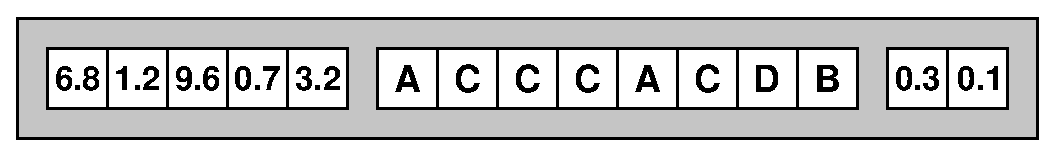
\includegraphics[scale=.5]{genom}
  \end{center}
%%  \centerline{   hans
%%      \psfig{figure=genom.eps,width=0.5\columnwidth}
%%  }
  \vspace{-15pt}\centerline{\parbox{13cm}{\caption[Representation of
    the Genome of an Individual]{Example for a representation of the
    genome of an individual consisting of three
    chromosomes.\label{datastruct:fig:genome-rep}}}}
\end{figure}

\begin{example}[hb]
\begin{shortlisting}
            \vdots\\
\#include <Individual.h>  // \textrm{declarations}\\
            \vdots\\
//\\
// {\rm define an individual with two chromosomes}\\
//\\
Individual indiv( ChromosomeT< bool   >( 80 ),\\
                  ChromosomeT< double >( 10 ) );\\
\\
//\\
// {\rm define range of values}\\
//\\
Interval range( -1.5, +3.0 );\\
\\
//\\
// {\rm initialize alleles of chromosome \#0}\\
//\\
dynamic\_cast< ChromosomeT< bool >\& >\\
    ( indiv[ 0 ] ).initialize( );\\
\\
//\\
// {\rm decode the binary values in chromosome \#0}\\
// {\rm to the floating point chromosome \#1}\\
//\\
dynamic\_cast< ChromosomeT< double >\& >\\
    ( indiv[ 1 ] ).decodeBinary( indiv[ 0 ], range, 10 );\hspace*{-10cm}\\
            \vdots\\
\end{shortlisting}
\vspace{-10pt}\centerline{\parbox{13cm}{\caption[Definition of a Sample Individual and Some Operations on its Genome]{
\label{datastruct:example:indiv-def}
Definition of a sample individual and some operations on its genome}}}
\end{example}



% =======================================================================
        \subsection{Populations}
% =======================================================================

A \myindex{population} represents a collection of individuals.  Individuals may
be sorted in a population either in ascending or descending order with
respect to their fitness. For class \verb+Population+ genetic
operators like \myindex{selection} and replacement are defined.  The \index{subscript
operator} $[\;]$ applied to a population returns the individual
specified by the index.  For a short example see
\exref{datastruct:example:pop-def}.
%% The operator $($ {\bf unsigned}, {\bf unsigned} $)$

\begin{example}[htb]
\begin{shortlisting}
            \vdots\\
\#include <Population.h>  // {\rm declarations}\\
            \vdots\\
//\\
// {\rm define population size}\\
//\\
const unsigned PopSize = 20;\\
\\
//\\
// {\rm define population with three chromosomes per individual}\\
//\\
Population pop( PopSize, ChromosomeT< char   >( 3 ),\\
                         ChromosomeT< int    >( 5 ),\\
                         ChromosomeT< double >( 8 ) ); \\
\\
//\\
// {\rm initialize alleles of chromosomes}\\
//\\
for( unsigned i = 0; i < pop.size( ); ++i ) \{\\
    dynamic\_cast( ChromosomeT< char >\& >\\
        ( pop[ i ][ 0 ] ).initialize( 'A', 'Z' );\\
    dynamic\_cast( ChromosomeT< int >\& >\\
        ( pop[ i ][ 1 ] ).initialize( -13,  10 );\\
    dynamic\_cast( ChromosomeT< double >\& >\\
        ( pop[ i ][ 2 ] ).initialize( 1.5, 4.5 );\\
\}\\
            \vdots\\
\end{shortlisting}
\vspace{-10pt}\centerline{\parbox{13cm}{\caption[Definition of a Sample Population with 20 Individuals]{\label{datastruct:example:pop-def}Definition of a sample population with 20 individuals.}}}
\end{example}
